\chapter{Validierung des Roboterdynamik-Modells}
\label{sec:modellvalidierung}
\label{cha:modellvalidierung}
%
Unter Berücksichtigung der getroffenen Annahmen wird untersucht, ob das implementierte Modell die Roboterdynamik hinreichend genau simuliert. Dazu werden die simulierten Drehmomente qualitativ und quantitativ mit den gemessenen Werten verglichen
%
\section{Messaufbau}
Als Testumgebung dient eine Roboterzelle in der digitalen Anlauffabrik des Mercedes-Benz Werks Berlin.
%Die Roboterzelle stellt einen von acht Laborbereichen zur Erprobung standardisierter Fertigungstechnologien dar.  
Der abgegrenzte Zellbereich ist mit Sicherheitseinrichtungen zur Gewährleistung der Personen- und Maschinensicherheit ausgestattet.
%sodass ein erheblich minimiertes Unfallrisiko in den Praxisversuchen gewährleistet ist. 
Der Roboter besitzt kein, am Flansch montiertes Werkzeug so dass das Kollisionsrisiko in den Versuchen im Vergleich zu einem Endeffektor (EE) mit komplexen Geometrien geringer ausfällt. Darüber hinaus ist eine signifikante Abweichung von der initialen Bahn durch Anwendung Bahnoptimierung wie in der Auswertung gezeigt nicht zu erwarten. Der Grund dafür hängt mit der Bahnplanung durch die Robotersteuerung zusammen. In der PTP-Bewegungsart berechnet die KR C5 den schnellsten Weg des Tool-Center-Point (TCP) zwischen Start- und Zielpunkt \cite[S.~429]{KSS.2023}. Eine stark abweichende Bahn im kartesischen Raum würde zu einem längeren Weg im Gelenkraum und damit zu einem höheren Energieverbrauch führen \cite[S.~59]{Eggers.2019}.
%5
%Ein Arbeitsgebiet der digitalen Anlauffabrik ist die Auswertung von prozessbezogenen Daten, sodass 
%
Der installierte KUKA KR 210 wird über eine KR C5 angesteuert, welche die KUKA RobotSensorInterface 5.0 (RSI) Technologie unterstützt. RSI ist eine Schnittstelle zur zyklischen Kommunikation zwischen dem Industrieroboter und einem Sensorsystem. Die Robotersteuerung kommuniziert mit dem Sensorsystem über eine echtzeitfähige Netzwerkverbindung. Die Daten werden dabei über das Ethernet UDP/IP-Protokoll \footnote{User Datagram Protocol (UDP) ist ein verbindungsloses Protokoll für den Datenaustausch von Netzwerkteilnehmern~\cite{RSI.2020}.} übertragen ~\cite[S.~11]{RSI.2020}. Der Roboter verfügt damit über eine Schnittstelle zur Aufzeichnung von Bewegungsdaten und den Messwerten interner Messeinrichtungen.  
%
Auf der Robotersteuerung ist daf{\"u}r ein RSI-Kontext zu parametrieren, wobei festgelegt wird, welche Daten an eine festgelegte Ziel-IP-Adresse inkl. Port {\"u}bertragen werden.~\cite[S.~43]{RSI.2020}.  Der Datenaustausch findet unidirektional zwischen zwei Netzwerkteilnehmern statt. Die KR C5 hat die Funktion eines sendenden Clients. Der Empfänger (Notebook) stellt den Server dar. Auf dem Empfänger wird die Ethernet Verbindung mit der definierten IP Adresse eingerichtet. Des Weiteren wird der im RSI Kontext festgelegte UDP-Port freigegeben. Der Port-Zugriff wird auf dem Windows Betriebssystem des Servers über die Programmierschnittstelle (Application Programming Interface(API)) Windows Sockets 2 (Winsock) realisiert \cite{Winsock.2023}. 
%
Der entsprechende RSI-Kontext wird im Initialisierungsschritt des KRL-Programms aktiviert \cite[S.~50]{RSI.2020}. Anschließend werden die Daten der erfassten Winkelverläufe und Drehmomente der einzelnen Gelenke in einem Takt von 4 ms in der American Standard Code for Information Interchange (ASCII) Darstellung an den Server übertragen. Die Daten werden in einem Textfile gespeichert und mithilfe der Skriptsprache Python in die JavaScript Object Notation (JSON) konvertiert, verarbeitet und visualisiert. 
%
Neben den Winkelverläufen werden die Winkelgeschwindigkeit, Winkelbeschleunigung, sowie die mechanische Leistung in den jeweiligen Gelenken benötigt. Da Winkelgeschwindigkeit und Winkelbeschleunigung nicht explizit zur Verfügung stehen, werden sie über den Differenzenquotient, siehe Kapitel \ref{sec:tarjektorie} gebildet. Durch Multiplikation der Winkelgeschwindigkeit mit dem Getriebe-Drehmoment wird der zeitliche Verlauf der mechanischen Leistung berechnet.

\section{Durchführung}
% Temperatur kalt und warm 
%Versuchsbeschreibung
Die Validierung des Modells erfolgt exemplarisch für die in der Tabelle \ref{tab:simu} definierte initiale Trajektorie aus dem Programm $Kleben-Seitenwand$. Die Betriebstemperatur des Roboters wird aufgrund der Vernachlässigung von Reibungseinflüssen im Modell nicht berücksichtigt. Die simulierten, sowie gemessenen Verläufe der Gelenkwinkel, Winkelgeschwindigkeit und Winkelbeschleunigung sind bereits im letzten Kapitel abgedruckt. Die simulierten Drehmomente werden in \ref{fig:taumat} gezeigt. Die gemessenen Werte sind in der Abbildung \ref{fig:tau} dargestellt. In beiden Fällen werden die Drehmomente auf der Getriebeseite betrachtet. Dies erfolgt mit dem Ziel die Zusammenhänge zwischen Drehmoment, Winkelgeschwindigkeit und mechanischer Leistung eindeutig erkennbar abzubilden. Eine Darstellung der Drehmomente auf der Motorseite wird vermieden. Durch Anwendung der Getriebe-Übersetzung ergibt sich eine Änderung des Vorzeichens der Momente in den Gelenken eins, zwei, vier und fünf, wie in Anhang \ref{add:systemparameter} angegeben, so dass die Zusammenhänge nicht ad hoc erkennbar sind.

\section{Auswertung}
Die gemessenen Drehmomente werden im Zeitintervall 0 s bis 1,3 s zu betrachtet. Daten für den Zeitraum $t>1,3~\text{s}$ entfallen auf den Vorgang der Antriebsregelung bis zum Einfallen der Haltebremsen, um den Roboter in Position zu halten. 
\subsection*{Quantitative Auswertung der Drehmomente}
Die simulierten Drehmomente fallen signifikant größer aus als die gemessenen. Der negative Maximalwert von $\tau_2$ liegt in der Simulation bei ca. -12 kNm. Dem gegenüber steht ein gemessener Wert  von ca. -2,8 kNm. Die Differenz wird der Vernachlässigung des Gewichtsausgleichs zugeschrieben. Dieser kompensiert insbesondere den Einfluss der Gewichtskraft nachfolgender Glieder am zweiten Gelenk. Exemplarisch zeigt Abbildung \ref{fig:gewichtskraft} den simulierten Anteil der Gewichtskraft bei Stillstand des Roboters in der Ausgangsstellung $q_{s,i}$ siehe Tabelle \ref{tab:simu}. Für die Drehmomente am zweiten Gelenk ist erkennbar, dass der Anteil der Gewichtskraft von -7743 Nm genau dem  Offset des Drehmoments beim Start der Bewegung entspricht. In der Konsequenz fällt $\tau_2$ im Gütekriterium der Optimierung zu stark ins Gewicht. Daraus wird abgeleitet, dass der Gewichtsausgleich in der Modellbildung zu berücksichtigen ist. 
%
\begin{figure}[tbph]
	\centering
	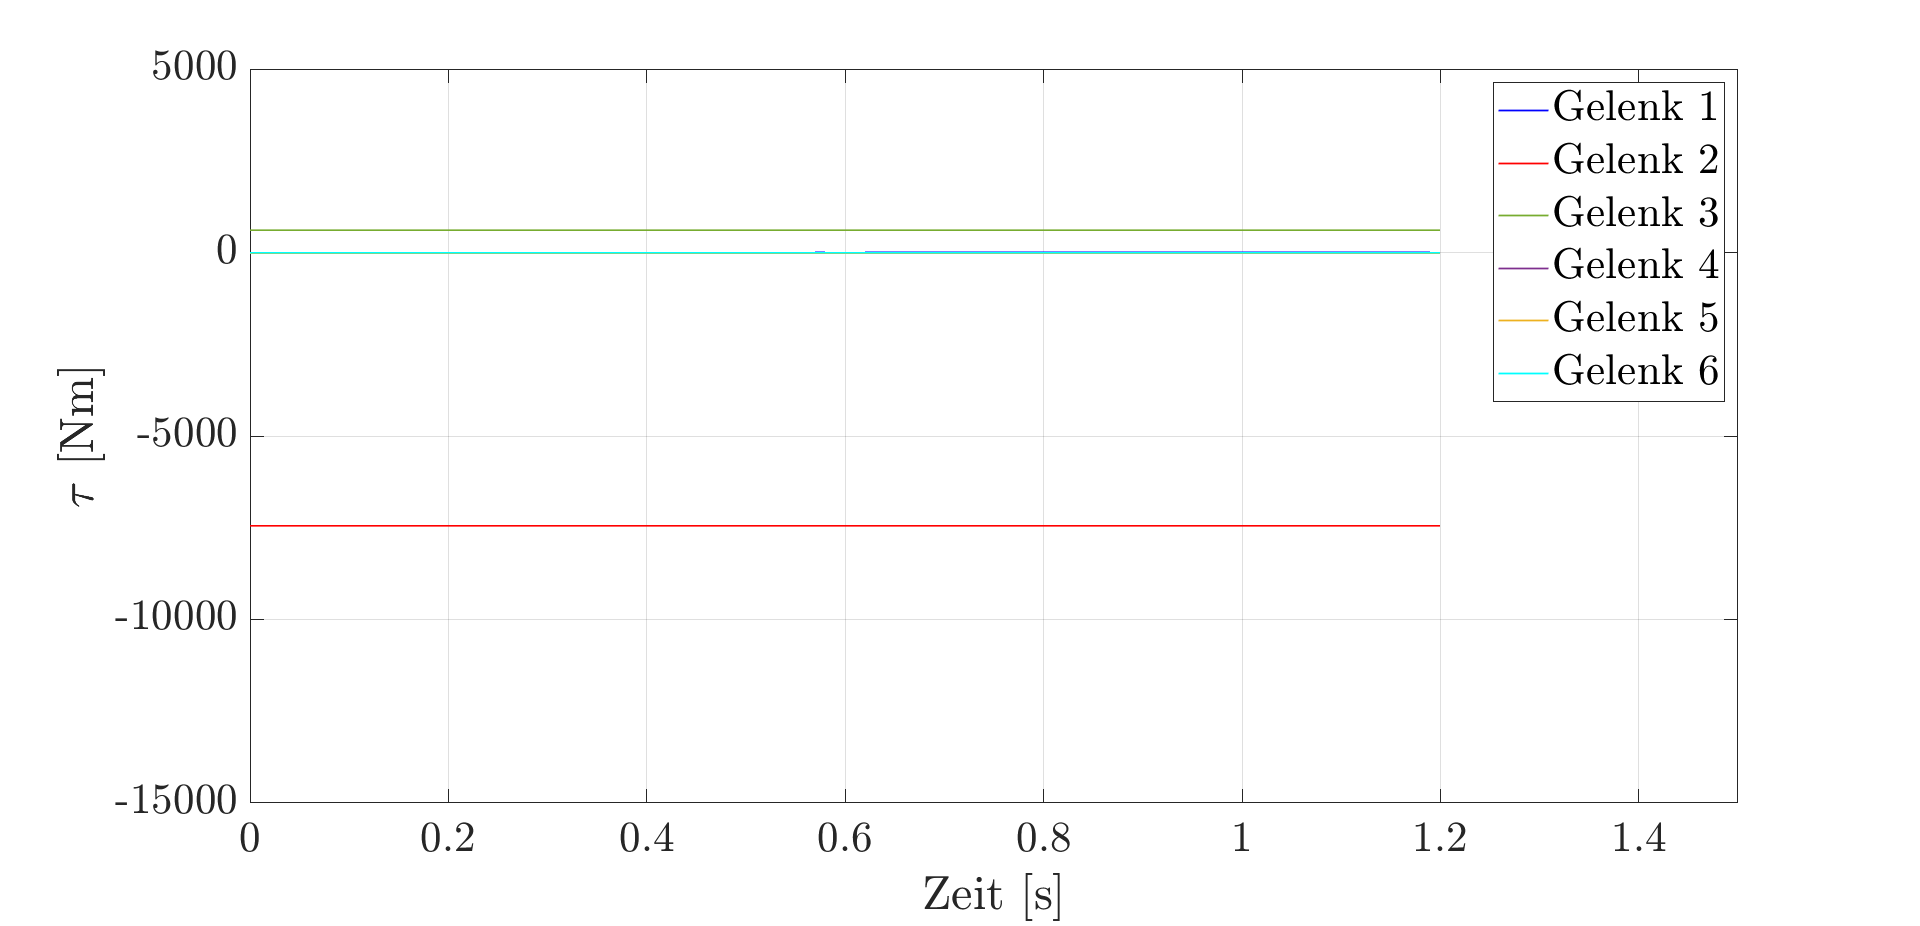
\includegraphics[width=1\linewidth]{images/Gewichtskraft}
	\caption{Anteil der Gewichtskraft an den Drehmomenten in der Startposition}
	\label{fig:gewichtskraft}
\end{figure}
%
%Idealerweise kompensiert der Ausgleichszylinder den Einfluss der Gewichtskraft aller nachfolgenden Glieder im zweiten Gelenk, siehe Abbildung \ref{fig:taumat-fgall}. 
%%
%\begin{figure}[tbph]
%	\centering
%	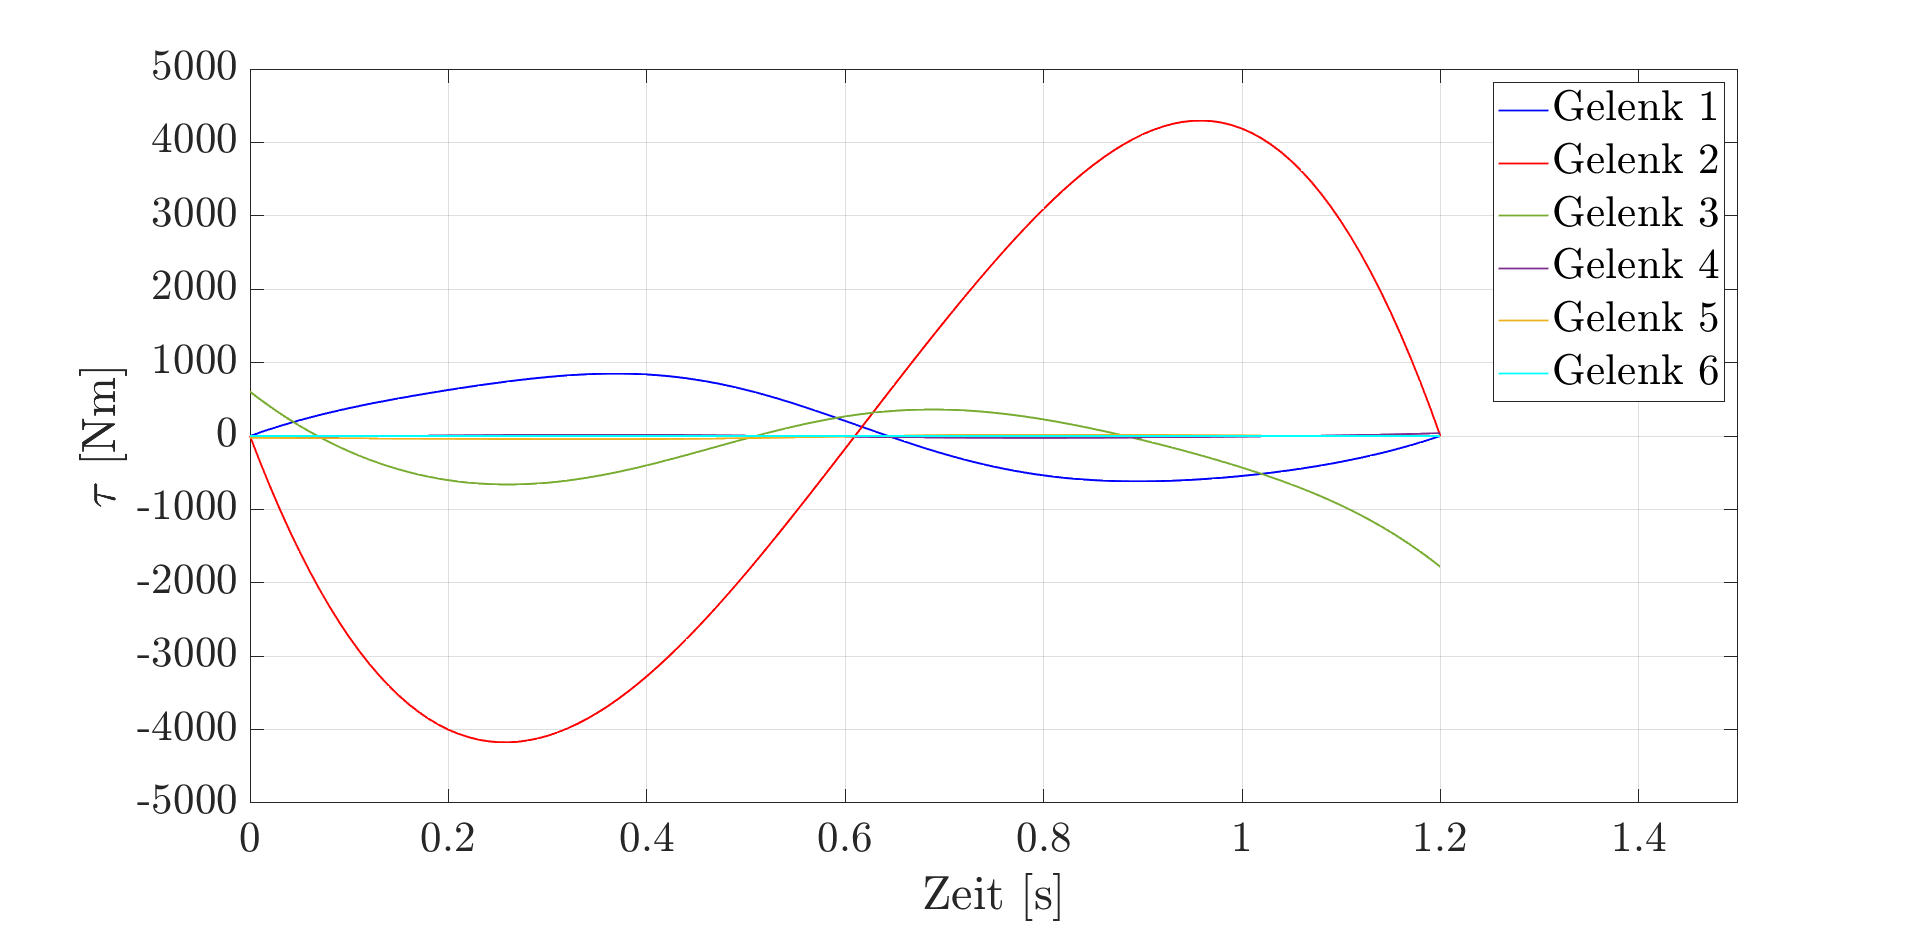
\includegraphics[width=1\linewidth]{images/taumat-fgall}
%	\caption{Drehmomentverlauf simuliert inkl. idealen Gewichtsausgleich}
%	\label{fig:taumat-fgall}
%\end{figure}
%
%Die Idealkompensation bildet jedoch nicht die Realität ab. Dies wird am Leistungsverlauf \ref{fig:p_ideal} gegenüber \ref{fig:p} nachgewiesen. 
%Es wird ein Kompromiss gewählt, bei dem ausschließlich die  Gewichtskraft des zweiten und dritten Verbindungsglieds ausgeglichen wird. 
Der Gewichtsausgleich wurde so gewählt, dass er den Anteils der Gewichtskraft des zweiten und dritten Verbindungsglieds am Drehmoment des zweiten Gelenks ausgleicht. 
Das Roboter-Dynamikmodell wird um die Vorschrift \ref{eqn:submugrav} erweitert.
%
\begin{equation}
	\label{eqn:submugrav}
\bm{\mu}^{i}_{i} = \bm{\mu}^{i}_{i} - {\bm{\mu}^{i}_{i}}_{grav} ~\forall ~i = 2
\end{equation}
%
wobei
%
\begin{equation}
	\label{eqn:mugrav}
	{\bm{\mu}^{i}_{i}}_{grav} = -{\bm{f}^{i}_{i}}_{grav} \times \left( \bm{r}^{i}_{i-1,i} + \bm{r}^{i}_{i,C_i} \right) + \bm{R}^{i}_{i+1} {\bm{\mu}^{i+1}_{i+1}}_{grav} + \bm{R}^{i}_{i+1} {\bm{f}^{i+1}_{i+1}}_{grav} \times \bm{r}^{i}_{i,C_i} ~\forall ~i = 2
\end{equation}
%
\begin{equation}
	\label{eqn:mugrav}
	{\bm{\mu}^{i}_{i}}_{grav} = -{\bm{f}^{i}_{i}}_{grav} \times \left( \bm{r}^{i}_{i-1,i} + \bm{r}^{i}_{i,C_i} \right) ~\forall ~i = 3
\end{equation}
%
\begin{equation}
	\label{eqn:subfgrav}
	{\bm{f}^{i}_{i}}_{grav} = \bm{R}^{i}_{i+1} {\bm{f}^{i+1}_{i+1}}_{grav} + m_i\ddot{\bm{p}}^{i}_{C_i} - {\bm{R}^0_i}^T - m_i \bm{g} ~\forall ~i \in \{2,3\}.
\end{equation}
%
Es folgt ein Drehmomentverlauf gemäß Abbildung \ref{fig:taumat-fg}. 
%
% Quelle Reibung Getriebe
%
\subsection*{Qualitative Auswertung der Drehmomente}
Die Gelenke werden nachfolgend einzeln betrachtet. Für das erste Gelenk weißt der gemessene Drehmomentverlauf einen steileren Anstieg als die simulierten Werte auf. Dieser Anstieg ist äquivalent zum Verlauf der Winkelbeschleunigung im selben Zeitabschnitt, siehe Abbildung \ref{fig:winkelbeschleunigung_py}. Das Maximum der simulierten Werte für das erste Gelenk ist ca. 50 \% kleiner als die gemessenen Werte. In der Ursache wird die Reibung des Getriebes vermutet. Der gemessene Drehmomentverlauf im ersten Gelenk weißt außerdem keinen negativen Anteil auf. Es wird angenommen, dass die Getriebemomente in der Signalaufzeichnung mithilfe von messtechnisch erfassten Motorströmen sowie der Drehmomentkonstanten und der Getriebeübersetzungsfaktoren berechnet werden. Unter der Annahme, dass die Bremsenergie nicht zurückgewonnen wird, sondern über Bremswiderstände dissipiert, entsprechen die gemessenen Werte für $t>0,8~\text{s}$ dem  Abbremsvorgang. Belegt wird dies mit dem übereinstimmenden Verlauf der Winkelgeschwindigkeit, siehe Abbildung \ref{fig:winkelgeschwindigkeit_py1}. Dass der Drehmomentverlauf dem Geschwindigkeitsverlauf dabei um ca. 0,02 s nachläuft, wird den Energie speichernden Induktivitäten der Antriebe zugeschrieben. Für den Drehmomentverlauf im zweiten Gelenk sind ebenfalls steilere Anstiege infolge eines höheren Rucks des realen Roboters festzustellen. Im Verlauf ist das negativen Maximum des simulierten Drehmoments im zweiten Gelenk ca. 2000 Nm größer als das aufgezeichnete Drehmoment des realen Systems. Die Differenz wird dem nur näherungsweise modellierten Gewichtsausgleich zugeschrieben. Aufgrund der kinematischen Kopplung wirkt der Einfluss des Gewichtsausgleichs am realen Roboter indirekt auch auf das dritte Gelenk womit der Offset zu Beginn der Bewegung erklärt wird. Dass die Größenordnung des Drehmoments im dritten Gelenk nicht erreicht wird, wird der Vernachlässigung der Stator-Massen von für die Motoren vier und fünf, der Rotor-Trägheit des dritten Motors, sowie und der Steifigkeit, Masse des Schlauchpakets zugeschrieben. Mit einem Gewicht von 65,3 kg ohne elektrische Leitungen steht die Masse des Schlauchpakets, gemäß CAD-Modell mindestens im Verhältnis 1:5 zur Masse des dritten Verbindungsglieds. Daraus folgt insbesondere eine zusätzliche Massenträgheit, sowie die Verschiebung des Masseschwerpunkts, unter der Annahme, dass die Hardware ausschließlich am dritten Verbindungsglied befestigt ist. Aufgrund fehlender Daten entfällt eine Berücksichtigung des Schlauchpakets. Des Weiteren wird für das Drehmoment im dritten Gelenk sowie die Drehmomente in allen nachfolgenden Gelenken die Vernachlässigung  der Reibungseffekte als Ursache für die erkennbare Abweichung gegenüber den Messdaten vermutet. 
%
\begin{figure}[tbph]
	\centering
	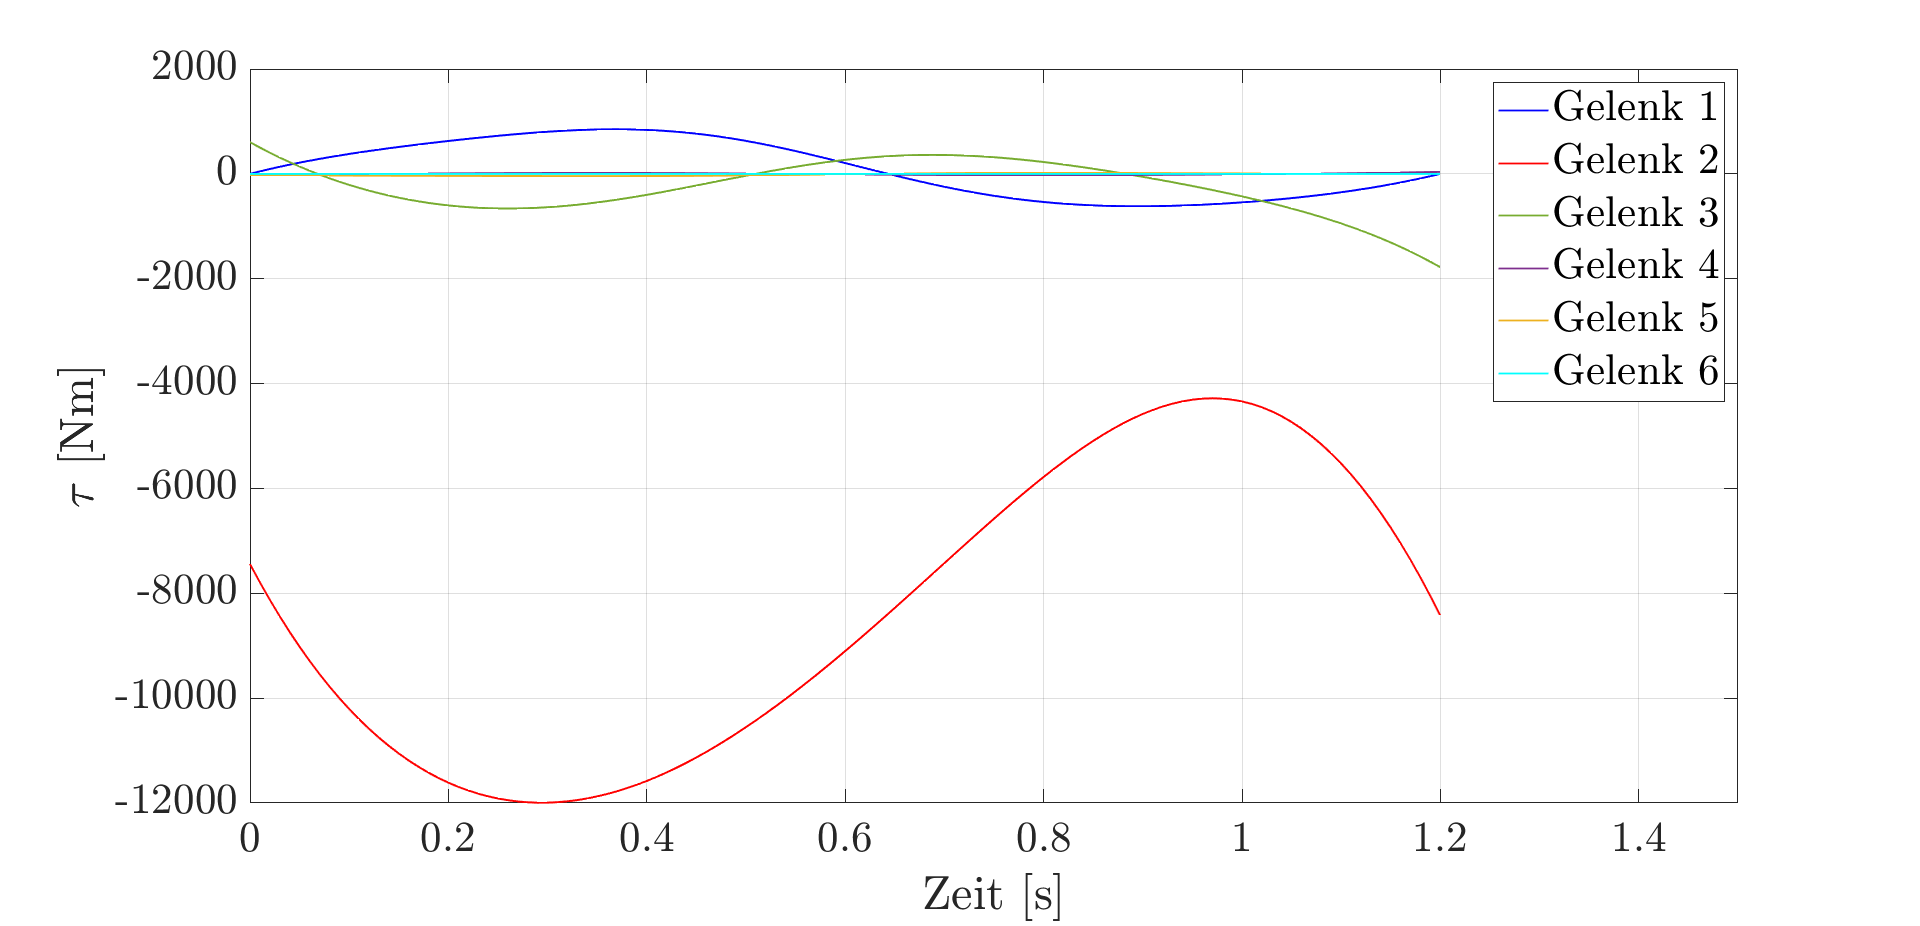
\includegraphics[width=1\linewidth]{images/taumat}
	\caption{Drehmomentverlauf simuliert ohne Gewichtsausgleich}
	\label{fig:taumat}
\end{figure}
%
\begin{figure}[tbph]
	\centering
	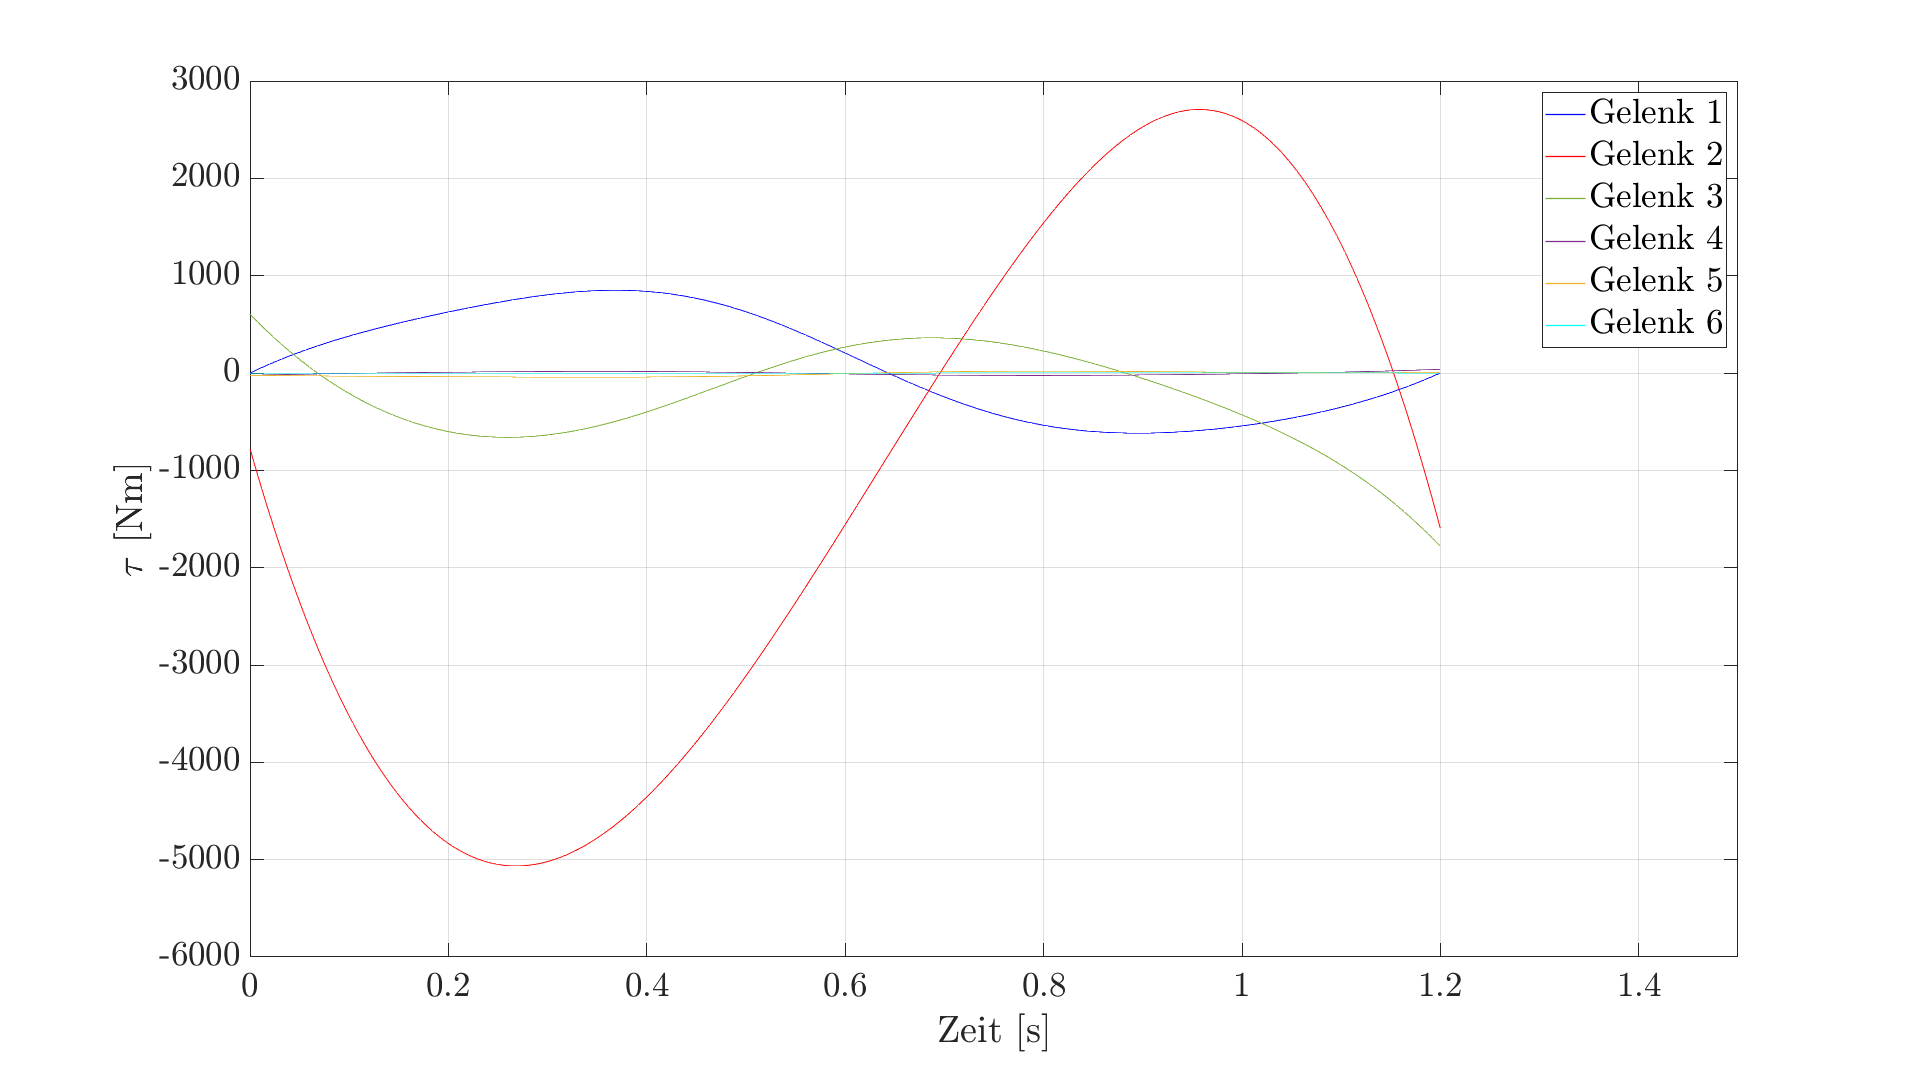
\includegraphics[width=0.9\linewidth]{images/taumat-fg}
	\caption{Drehmomentverlauf simuliert inkl. näherungsweise modellierten Gewichtsausgleich}
	\label{fig:taumat-fg}
\end{figure}
%
\begin{figure}[tbph]
	\centering
	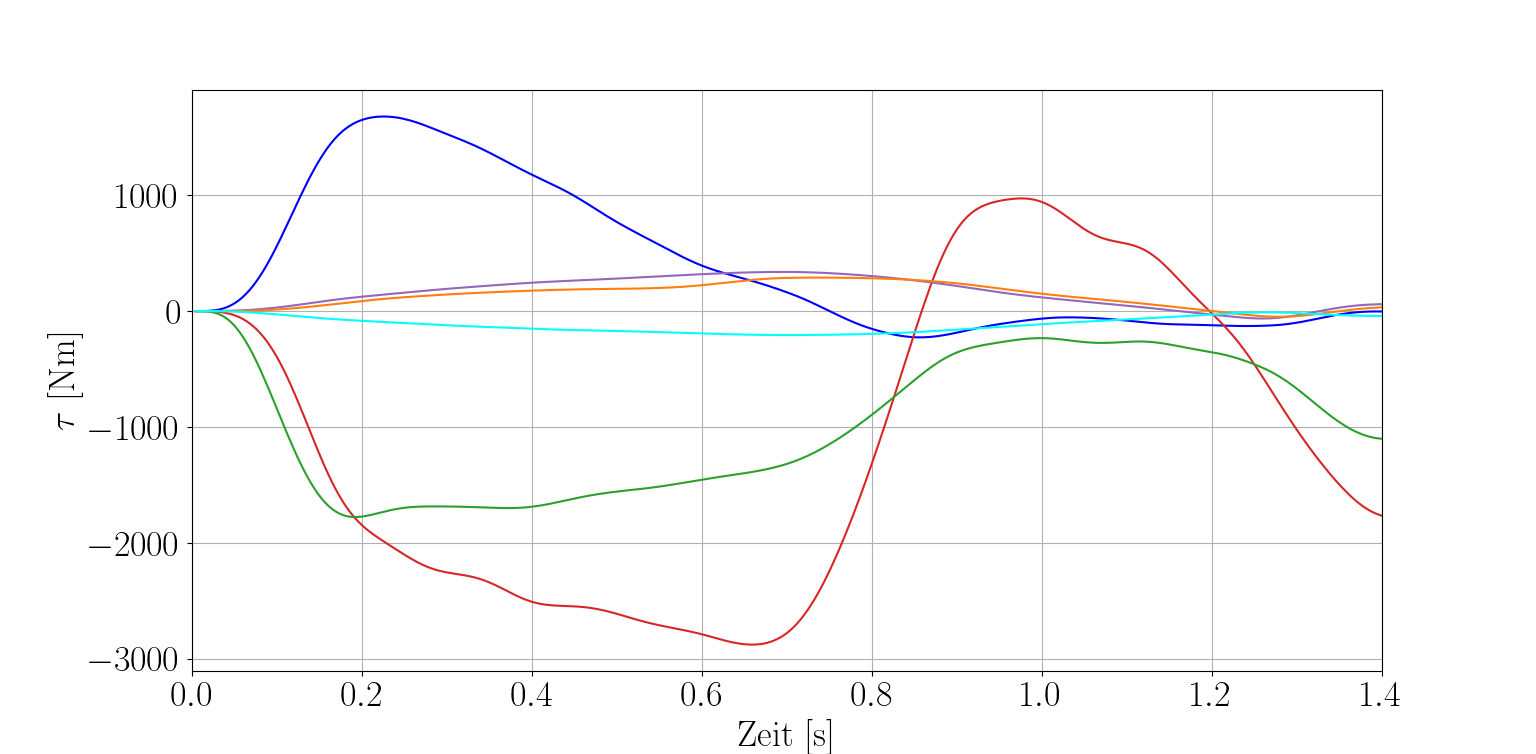
\includegraphics[width=1\linewidth]{images/tau}
	\caption{Drehmomentverlauf gemessen}
	\label{fig:tau}
\end{figure}
%
\subsection*{Auswertung der mechanischen Leistung}
Die simulierten Leistungsdaten des ersten Gelenks stimmen in etwa mit den Werten überein, die auf der Grundlage der RSI Daten berechnet wurden. Der simulierte Verlauf der mechanischen Leistung für das zweite Gelenk weist einen ähnlichen Verlauf wie die messtechnisch erfassten Werte auf. Der Nulldurchgang der gemessenen Leistungskurve ist um 1,3 Sekunden nach rechts verschoben.  Dies lässt sich unter Berücksichtigung der RSI-Daten zur Winkelbeschleunigung in Abbildung \ref{fig:winkelbeschleunigung_py} auf die kürzere Abbremsdauer des realen Roboters gegenüber der im Modell implementierten Bahnplanung  zurückführen. In der gezeigten Bewegung wird die mechanische Leistung in den anderen Antrieben nicht durch das Modell abgebildet. Infolgedessen liegt der Schwerpunkt der Optimierung auf der Anpassung der Roboterkonfiguration zugunsten des Drehmoments im zweiten Gelenk. 
%
\begin{figure}[tbph]
	\centering
	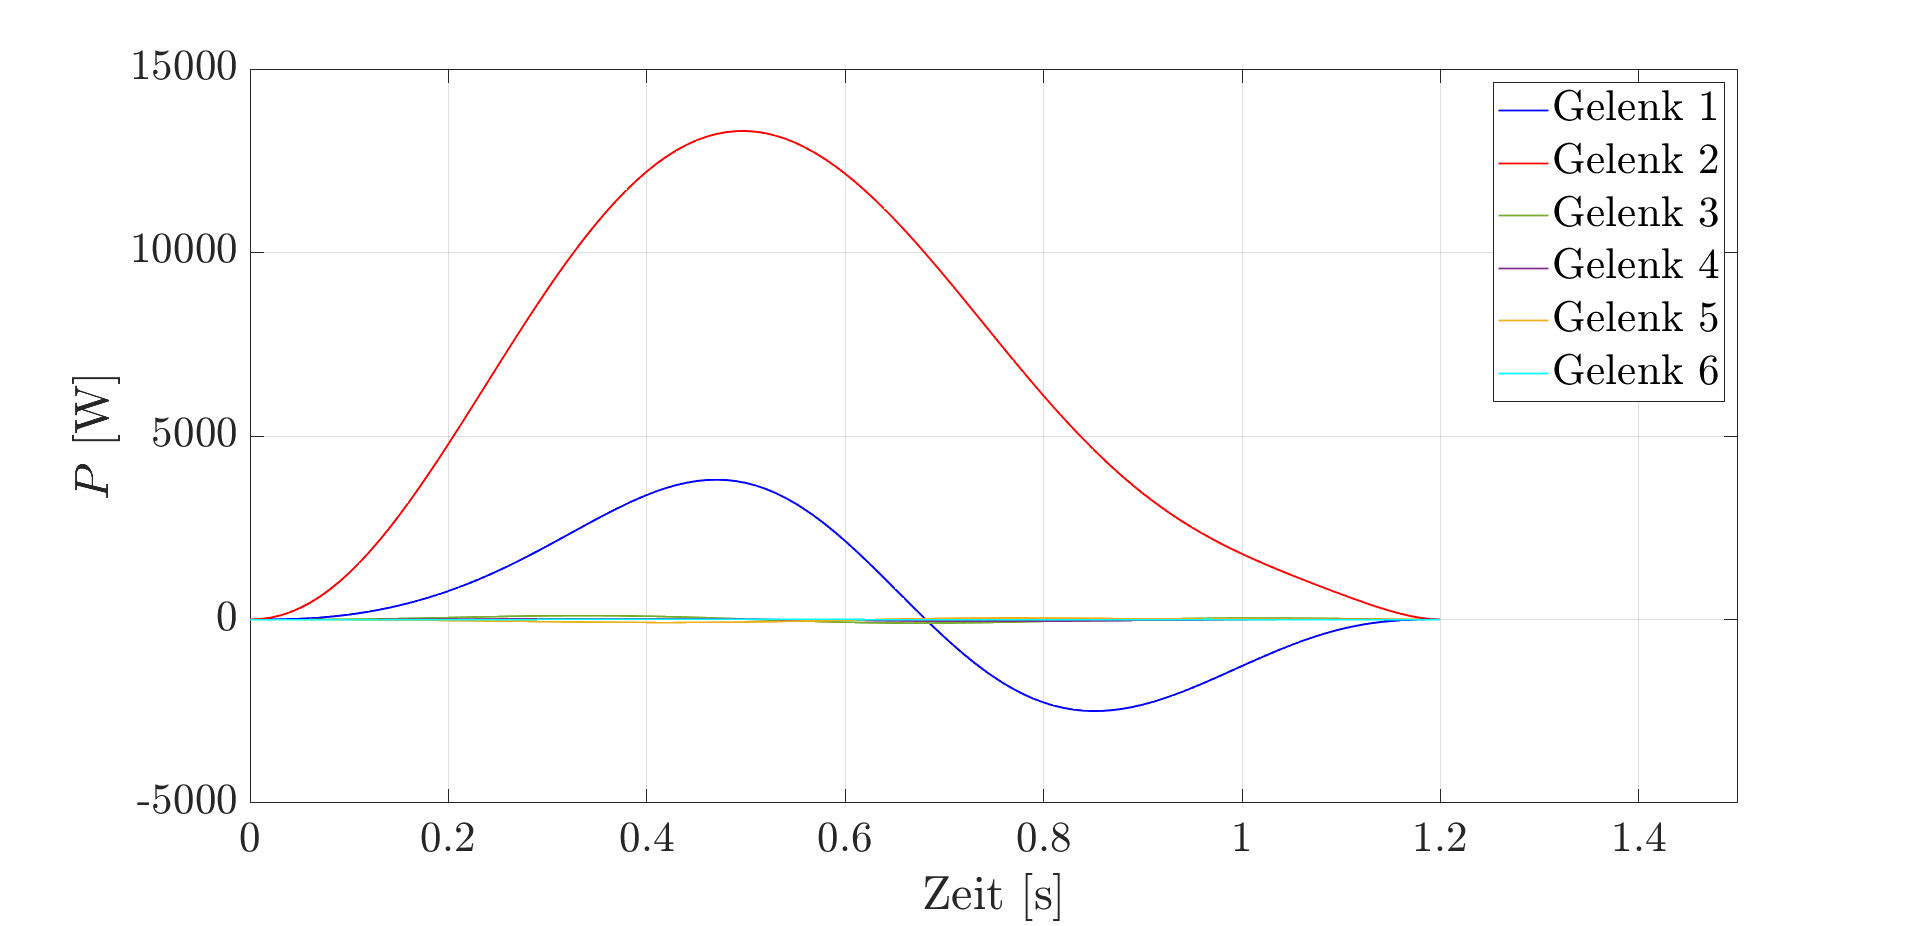
\includegraphics[width=1\linewidth]{images/pmat}
	\caption{mechanische Leistung simuliert}
	\label{fig:pmat}
\end{figure}
%
\begin{figure}[tbph]
	\centering
	\includegraphics[width=1\linewidth]{images/p}
	\caption{mechanische Leistung gemessen}
	\label{fig:p}
\end{figure}
%
\subsection*{Schlussfolgerung}
Es wurde die Qualität eines Modells zur Simulation der mechanischen Leistungsaufnahme des Roboters für eine Bewegung mit der Start- und Zielkonfiguration gemäß Tabelle \ref{tab:simu} untersucht. Die ausgewählte Bahn entspricht dem Verfahrweg des Roboters vom letzten Prozesspunkt zur Grundstellung im Fertigungsprogramm $Kleben-Seitenwand$. Aufgrund des hohen Anteils der gemessenen sowie simulierten mechanischen Leistung für das zweite Gelenk im Vergleich zu den anderen Gelenken wird das größte Optimierungspotenzial im Modell berücksichtigt. Für die untersuchte Bewegung erfüllt das Modell den Zweck der Zielfunktionsberechnung zur Optimierung der ausgewählten Bewegungsbahn.
%